% Plantilla LaTeX para informe de estudio científico
% Archivo: informe.tex
% Compilación recomendada: pdflatex informe.tex -> biber informe -> pdflatex informe.tex (o use latexmk -pdf)

\documentclass[12pt,a4paper]{article}

% -------------------- Paquetes --------------------
\usepackage[utf8]{inputenc}        % codificación UTF-8
\usepackage[T1]{fontenc}
\usepackage[spanish]{babel}        % idioma español
\usepackage{csquotes}              % citas correctas con biblatex
\usepackage{geometry}              % márgenes
\usepackage{graphicx}              % incluir imágenes
\usepackage{caption,subcaption}    % subtítulos para figuras
\usepackage{booktabs}              % tablas bonitas
\usepackage{amsmath,amssymb}       % símbolos matemáticos
\usepackage{siunitx}               % unidades y números
\usepackage{float}                 % control de float
\usepackage{hyperref}              % enlaces
\usepackage{lineno}                % numerar líneas (opcional)
\usepackage{authblk}               % afiliaciones de autores
\usepackage{enumitem}              % listas con control
\usepackage{microtype}             % mejor tipografía
\usepackage{setspace}              % interlineado
\usepackage{longtable}             % tablas largas
\usepackage{appendix}              % apéndices

% Bibliografía con biblatex (usa biber)
\usepackage[backend=biber,style=apa,sorting=nyt]{biblatex}
\addbibresource{bibliografia.bib} % archivo .bib (crear bibliografia.bib)

% -------------------- Márgenes y formato --------------------
\geometry{left=30mm,right=25mm,top=30mm,bottom=30mm}
\setlength{\parskip}{0.5em}
\setlength{\parindent}{0pt} % sin sangría en párrafos
\onehalfspacing % interlineado 1.5 (cambiar por \singlespacing o \doublespacing)

% -------------------- Configuración personalizada para lstlisting --------------------
\usepackage{listings}
\usepackage{xcolor}

\lstdefinestyle{custompython}{
    language=Python,
    inputencoding=utf8,
    extendedchars=true,
    literate=
        {á}{{\'a}}1
        {é}{{\'e}}1
        {í}{{\'i}}1
        {ó}{{\'o}}1
        {ú}{{\'u}}1
        {Á}{{\'A}}1
        {É}{{\'E}}1
        {Í}{{\'I}}1
        {Ó}{{\'O}}1
        {Ú}{{\'U}}1
        {ñ}{{\~n}}1
        {Ñ}{{\~N}}1
        {ü}{{\"u}}1
        {Ü}{{\"U}}1,
    frame=single,
    frameround=tttt,
    rulecolor=\color{gray!70},
    backgroundcolor=\color{gray!10},
    basicstyle=\ttfamily\footnotesize,
    keywordstyle=\color{blue}\bfseries,
    stringstyle=\color{orange},
    commentstyle=\color{green!60!black}\itshape,
    numberstyle=\tiny\color{gray},
    numbers=left,
    stepnumber=1,
    numbersep=8pt,
    showstringspaces=false,
    tabsize=4,
    breaklines=true,
    breakatwhitespace=true,
    captionpos=b,
    morekeywords={as,with,try,except,finally,lambda,print,exit},
}

\lstset{style=custompython}

% Información del documento
\title{Informe de Resolución de Modelo Dinámico Complejo}
\author[1]{Ismael Sallami Moreno}
\author[2]{David Bacas Posadas}
\affil[1]{Doble Grado en Ingeniería Informática y Administración y Dirección de Empresas, Universidad de Granada, España}
\date{Fecha del informe: \today}

% -------------------- Inicio del documento --------------------
\begin{document}
\maketitle
% \begin{abstract}
%   Resumen breve (150--250 palabras). Indicar objetivo, método principal, resultados clave y conclusión breve.
% \end{abstract}

% Palabras clave
% \vspace{1em}
% \noindent\textbf{Palabras clave:} palabra1; palabra2; palabra3

% Numerar líneas si se desea (útil para revisores)
% \linenumbers

% -------------------- Secciones principales --------------------
\section{Introducción}
En el presente documento vamos a detallar la resolución de un modelo dinámico complejo basándonos en un estudio de la Universidad de Almería, la cual relaciona el comportamiento de diferentes variables en un sistema dinámico físico con la crisis que se produjo en el pasado. Este documento es un borrador, por ende, va a ser breve y poco detallado.

\section{Resumen del estudio de partida}

El estudio de los de Almería, titulado \textbf{"Diffusive and Arrestedlike Dynamics in Currency Exchange Markets"}, investigó la analogía entre la dinámica de los fluidos y vidrios (partículas coloidales en estados sobreenfriados o detenidos) y la dinámica del mercado de divisas Euro-Dólar estadounidense (EURUSD).

El estudio fue publicado en \emph{Physical Review Letters} en 2017 y fue realizado por J. Clara-Rahola, A. M. Puertas, M. A. Sánchez-Granero, J. E. Trinidad-Segovia, y F. J. de las Nieves, con afiliaciones a la Universidad de Almería y otras instituciones.

\subsection*{Hallazgos Principales}

\begin{itemize}
    \item \textbf{Simetría con la física de vidrios:} El estudio encontró una simetría significativa entre las distribuciones de fluctuación del precio del EURUSD y las de partículas coloidales en sistemas detenidos o sobreenfriados.
    \item \textbf{Dinámica a largo plazo (Anual):} Al promediar los datos a lo largo de los años, el \emph{Desplazamiento Cuadrático Medio del Precio} (MSPD, análogo al MSD en física) mostró un comportamiento \textbf{difusivo} (lineal) en todo momento.
    \item \textbf{Dinámica Contextual (Diaria):} Se encontró una dinámica de \textbf{detención temporal} (similar a la de vidrios) al enfocarse en marcos de tiempo diarios específicos, especialmente cuando cierra el mercado de Nueva York (alrededor de las 6:00 p.m. ET). Esta dinámica se caracteriza por un MSPD de dos pasos (una meseta intermedia).
    \item \textbf{Parámetros de Verificación:} La analogía se corroboró con el análisis del factor de estructura dinámico ($S(q, \tau)$) y el parámetro no gaussiano ($\alpha_2(\tau)$), que mostraron el comportamiento típico de fluidos sobreenfriados.
\end{itemize}

\subsection*{Fórmulas Clave}

El estudio adaptó un modelo de la física de vidrios (la función de van Hove) para describir la \emph{Función de Distribución de Probabilidad} (PDF) de las fluctuaciones del precio ($\delta p(\tau)$). La función original se modificó para incorporar difusión a corto plazo, utilizando un proceso de Ornstein-Uhlenbeck para la componente vibracional $f_{vib}(p, t)$.

\begin{enumerate}
    \item \textbf{Función de Distribución de Desplazamiento (Van Hove Modificada):}

    Donde $f_{vib}(p)$ se sustituye por la función de Ornstein-Uhlenbeck, $FT^{-1}$ es la transformada inversa de Fourier, $\tilde{f}(q) = \tilde{f}_{vib}(q)\tilde{f}_{jump}(q)$ es el factor de estructura dinámico, $\tau_{1}$ es el tiempo de salto para la primera vez y $\tau_{2}$ para saltos posteriores:

    $$
    G(p,t) = \tau_{1}f_{vib}(p)\phi_{1}(t) + FT^{-1}\left(\tilde{f}_{vib}(q)\tilde{f}(q)\tau_{2}\frac{\exp\{[\tilde{f}(q)-1]t/\tau_{2}\}-\exp(-t/\tau_{1})}{\tau_{2}-\tau_{1}+\tilde{f}(q)\tau_{1}}\right)
    $$

    \item \textbf{Distribución de Ornstein-Uhlenbeck para la Componente Vibracional ($f_{vib}(p, t)$):}

    Donde $D$ es el coeficiente de difusión y $\alpha = D/l^2$ con $l$ siendo el tamaño de la jaula:

    $$
    f_{vib}(p,t) = \sqrt{\frac{\alpha}{2\pi D(1-e^{-2\alpha t})}}\exp\left\{-\frac{\alpha p^{2}}{2D(1-e^{-2\alpha t})}\right\}
    $$

    \item \textbf{Desplazamiento Cuadrático Medio del Precio (MSPD):}

    Análogo al MSD en física, $\tau$ es el tiempo de retardo:

    $$
    \langle\Delta p^{2}(\tau)\rangle=\langle[p(t_{0}+\tau)-p(t_{0})]^{2}\rangle
    $$

    \item \textbf{Parámetro No-Gaussiano ($\alpha_2(\tau)$):}

    Cuantifica la desviación de la PDF con respecto a la gaussiana:

    $$
    \alpha_{2}(\tau)=\frac{\langle\Delta p(\tau)^{4}\rangle}{3\langle\Delta p(\tau)^{2}\rangle^{2}}-1
    $$
\end{enumerate}

\section{Datos Escogidos: Greece-Germany}

El uso del diferencial \textbf{Grecia-Alemania} (o \emph{spread}) no es una elección arbitraria, sino una necesidad metodológica y académica que se alinea directamente con el objetivo del estudio de \textbf{Econofísica} y el contexto de la \textbf{crisis de la deuda soberana europea}, tal como se infiere del documento de la Universidad de Almería.

\subsection*{Justificación del Uso del Spread Grecia-Alemania}

\begin{enumerate}[label=\arabic*.]
    \item \textbf{Representación de la Dinámica de No Equilibrio (Econofísica):} El núcleo de la Econofísica es aplicar herramientas de la Física Estadística a sistemas financieros en estado de no equilibrio. El spread Grecia-Alemania es la métrica directa del riesgo de quiebra soberana percibido en Grecia relativo al activo más seguro de la Eurozona (Alemania). Esta serie temporal está sujeta a shocks y periodos de alta tensión que desencadenan la dinámica de arresto o fase vítrea que el modelo MSPD busca identificar.
    \item \textbf{Roles Asimétricos dentro de la Eurozona:} Grecia representa el país en el epicentro de la crisis de deuda soberana, mientras que Alemania es el activo "libre de riesgo" de la Eurozona. El spread entre ambos países refleja la máxima prima de riesgo y sirve como indicador de tensión financiera.
    \item \textbf{Coherencia con la Metodología Académica:} La literatura académica y el documento original centran el análisis en diferenciales entre el país más afectado por la crisis y el país con la deuda más segura. El spread Grecia-Alemania permite aislar y analizar los efectos de no equilibrio sobre el activo soberano más vulnerable.
    \item \textbf{Alternativas Descartadas:} Otros spreads, como Francia-Alemania o España-Italia, no presentan la volatilidad ni la asimetría de riesgo necesarias para detectar fenómenos de lenta relajación y memoria en el mercado.
\end{enumerate}

En resumen, la selección del spread Grecia-Alemania es el caso de estudio ideal para replicar la metodología de la Econofísica y detectar las dinámicas de memoria que surgen durante una crisis sistémica.

Para conseguir los datos, se ha servido de la web \href{https://es.investing.com/rates-bonds/de-10y-vs-gr-10y-historical-data}{investing}. En cuanto a las fechas seleccionadas, se han escogido desde el 1 de enero de 2008 hasta el 31 de diciembre de 2018, ya que cubren el periodo de la crisis financiera global y la crisis de deuda soberana europea. Para pruebas más rápidas, se puede reducir el rango de fechas, parte para la cual se ha añadido una parte en el script de Python para mejorar la robustez en la lectura de pocos datos.

Se ha usado dos archivos CSV, uno de la actualidad para ver si la parte general funciona, además poniendo a prueba la parte de robustez de pocos datos y otra parte que cubre todo el periodo de la crisis.

\section{Análisis del Código}

\subsection{Código principal de análisis de spread Grecia-Alemania}

A continuación se muestra el código Python utilizado para analizar el spread de bonos entre Grecia y Alemania, calcular el MSPD, ajustar una ley de potencia y aplicar un modelo GARCH. El código también genera y guarda gráficos de los resultados.

\begin{lstlisting}[language=Python, caption={Análisis Econofísico y Econométrico del Spread Grecia-Alemania}]
import pandas as pd
import numpy as np
import matplotlib.pyplot as plt
from scipy.optimize import curve_fit
from arch import arch_model
import warnings
import os 

# --- NOMBRES DE COLUMNAS A BUSCAR Y ARCHIVO ---
COLUMNA_FECHA_BUSQUEDA = 'Fecha'  
COLUMNA_SPREAD = 'Último'         
ARCHIVO_DATOS = "GREECE-GERMANY-SPREAD-BONOS.csv"
OUTPUT_DIR = 'image' # 

warnings.filterwarnings('ignore')

# FASE 1: CARGA Y PREPARACIÓN DE DATOS REALES
try:
    try:
        df = pd.read_csv(ARCHIVO_DATOS, encoding='utf-8') 
    except UnicodeDecodeError:
        df = pd.read_csv(ARCHIVO_DATOS, encoding='latin1')
    columnas_limpias = df.columns.str.strip().str.replace('\ufeff', '')
    df.columns = columnas_limpias
    if df.columns[0] != COLUMNA_FECHA_BUSQUEDA:
        df = df.rename(columns={df.columns[0]: COLUMNA_FECHA_BUSQUEDA})
    df = df.set_index(COLUMNA_FECHA_BUSQUEDA)
    df.index = pd.to_datetime(df.index, errors='coerce', dayfirst=True)
    df['Spread_str'] = df[COLUMNA_SPREAD].astype(str)
    df['Spread'] = df['Spread_str'].str.replace('.', '', regex=False).str.replace(',', '.', regex=False)
    df['Spread'] = pd.to_numeric(df['Spread'], errors='coerce')
    df = df.dropna(subset=['Spread']) 
    p_t = df['Spread'].values 
    df['Retornos'] = df['Spread'].pct_change()
    retornos = df['Retornos'].dropna().values
except Exception as e:
    print(f"ERROR FATAL: La lectura falló. Mensaje final: {e}")
    exit()

# FASE 2: CÁLCULO DEL MSPD Y AJUSTE POWER LAW
def calcular_mspd(p_t, max_tau=252):
    N = len(p_t)
    mspd_results = {}
    for tau in range(1, max_tau + 1):
        if N - tau <= 0: break
        squared_displacements = (p_t[tau:] - p_t[:-tau])**2
        mspd_results[tau] = np.mean(squared_displacements)
    return pd.Series(mspd_results)

def power_law(tau, A, alpha):
    return A * (tau ** alpha)

mspd_df = calcular_mspd(p_t, max_tau=min(252, len(p_t)//2))
tau_values = mspd_df.index.values
mspd_values = mspd_df.values
alpha_fit = np.nan 

try:
    fit_range = len(tau_values) // 2 
    params, cov = curve_fit(power_law, tau_values[:fit_range], mspd_values[:fit_range], p0=[1, 1], maxfev=5000)
    A_fit, alpha_fit = params
    fit_curve = power_law(tau_values, A_fit, alpha_fit)
except RuntimeError:
    pass

# FASE 3: MODELO GARCH
if len(retornos) < 100:
    alpha_1 = np.nan
    beta_1 = np.nan
else:
    try:
        am = arch_model(retornos * 100, mean='Constant', vol='Garch', p=1, q=1, dist='StudentsT')
        res = am.fit(update_freq=5, disp='off')
        if 'arch[1]' in res.params and 'garch[1]' in res.params:
            alpha_1 = res.params['arch[1]']
            beta_1 = res.params['garch[1]']
        else:
            alpha_1 = np.nan
            beta_1 = np.nan
    except Exception as e:
        alpha_1 = np.nan
        beta_1 = np.nan

# FASE 4: VISUALIZACIÓN Y GUARDADO DE RESULTADOS
if not os.path.exists(OUTPUT_DIR):
    os.makedirs(OUTPUT_DIR)

plt.figure(figsize=(14, 6))
plt.plot(df.index, df['Spread'], label='Spread de Bonos Grecia-Alemania', color='tab:blue')
plt.title('1. Serie Temporal del Spread de Bonos (Grecia-Alemania)')
plt.xlabel('Fecha')
plt.ylabel('Spread (puntos base)')
plt.grid(True, linestyle='--', alpha=0.6)
plt.savefig(os.path.join(OUTPUT_DIR, '1_Serie_Temporal_Spread.png'))
plt.close()

plt.figure(figsize=(10, 8))
plt.loglog(tau_values, mspd_values, 'o', label='MSPD (Datos Reales)')
if not np.isnan(alpha_fit):
    plt.loglog(tau_values, fit_curve, '-', label=f'Ajuste Power Law (\alpha={alpha_fit:.2f})', color='red')
    power_law_difusivo = power_law(tau_values, A_fit, 1.0)
    plt.loglog(tau_values, power_law_difusivo, '--', label=r'Referencia $\alpha=1$ (Difusivo)', color='gray')
plt.title('2. Desplazamiento Cuadrático Medio del Precio (MSPD) - Escala Log-Log')
plt.xlabel(r'Lag Time $\tau$ (días) - Log Scale')
plt.ylabel(r'MSPD $\langle \Delta p^2(\tau) \rangle$ - Log Scale')
plt.legend()
plt.grid(True, which="both", ls="--")
plt.savefig(os.path.join(OUTPUT_DIR, '2_MSPD_Log_Log.png'))
plt.close()
\end{lstlisting}

\subsection{Explicación paso a paso del código}

\begin{enumerate}
    \item \textbf{Carga y limpieza de datos:} Se lee el archivo CSV con los datos del spread, se limpian los encabezados y se convierte el formato de los valores para asegurar la correcta interpretación numérica.
    \item \textbf{Preparación de la serie temporal:} Se extrae la columna de spread y se calcula la serie de retornos porcentuales diarios.
    \item \textbf{Cálculo del MSPD:} Se implementa una función que calcula el desplazamiento cuadrático medio del precio para distintos valores de retardo ($\tau$), siguiendo la metodología de econofísica.
    \item \textbf{Ajuste de ley de potencia:} Se ajusta el MSPD calculado a una función de ley de potencia para estimar el exponente de escala $\alpha$, que indica el tipo de dinámica (difusiva, subdifusiva, etc.).
    \item \textbf{Modelo econométrico GARCH:} Si hay suficientes datos, se ajusta un modelo GARCH(1,1) para analizar la persistencia de la volatilidad en los retornos del spread.
    \item \textbf{Visualización y guardado de resultados:} Se generan dos gráficos: la serie temporal del spread y el MSPD en escala log-log, guardándolos en la carpeta \texttt{image}.
\end{enumerate}

\subsubsection{¿Qué es el modelo GARCH?}

El modelo GARCH (Generalized Autoregressive Conditional Heteroskedasticity) es un modelo estadístico utilizado para analizar y predecir la volatilidad en series temporales financieras. Fue desarrollado por Tim Bollerslev en 1986 como una extensión del modelo ARCH (Autoregressive Conditional Heteroskedasticity) propuesto por Robert Engle en 1982.

El modelo GARCH captura la característica de heterocedasticidad condicional, que se refiere a la variabilidad de la volatilidad a lo largo del tiempo. En otras palabras, el modelo asume que la volatilidad actual depende de los valores pasados de la volatilidad y de los errores pasados.

\section{Salida del período de la crisis y análisis de resultados}

Al ejecutarlo nos da la siguiente salida:
\begin{verbatim}
python3 econofisica_spread_model.py
--- FASE 1: CARGANDO DATOS DESDE datos-largos.csv ---
--- APLICANDO SOLUCIÓN ROBUSTA: Limpieza de encabezados y formato decimal ---
Lectura exitosa.
Período analizado: 2016-03-04 a 2018-12-31 | Puntos: 685

--- FASE 2: ANÁLISIS ECONOFÍSICO (MSPD) ---
Exponente de Escala (alpha): 0.7857
  -> Interpretación: Subdifusivo (Arresto Dinámico/Memoria Lenta)

--- FASE 3: MODELO ECONOMÉTRICO (GARCH) ---
ERROR DE GARCH: El modelo no convergió y no se encontraron los parámetros.

--- FASE 4: GENERANDO Y GUARDANDO GRÁFICOS ---
 Gráficos guardados en la carpeta 'image'.

¡Ejecución completada! Analice los resultados y los gráficos generados.
\end{verbatim}

Vemos que el período analizado es desde el 4 de marzo de 2016 hasta el 31 de diciembre de 2018, con un total de 685 puntos de datos. Suponemos que la web de los datos no tiene datos anteriores a esa fecha. Esta parte se podría mejorar buscando otra fuente de datos.

\begin{figure}[H]
    \centering
    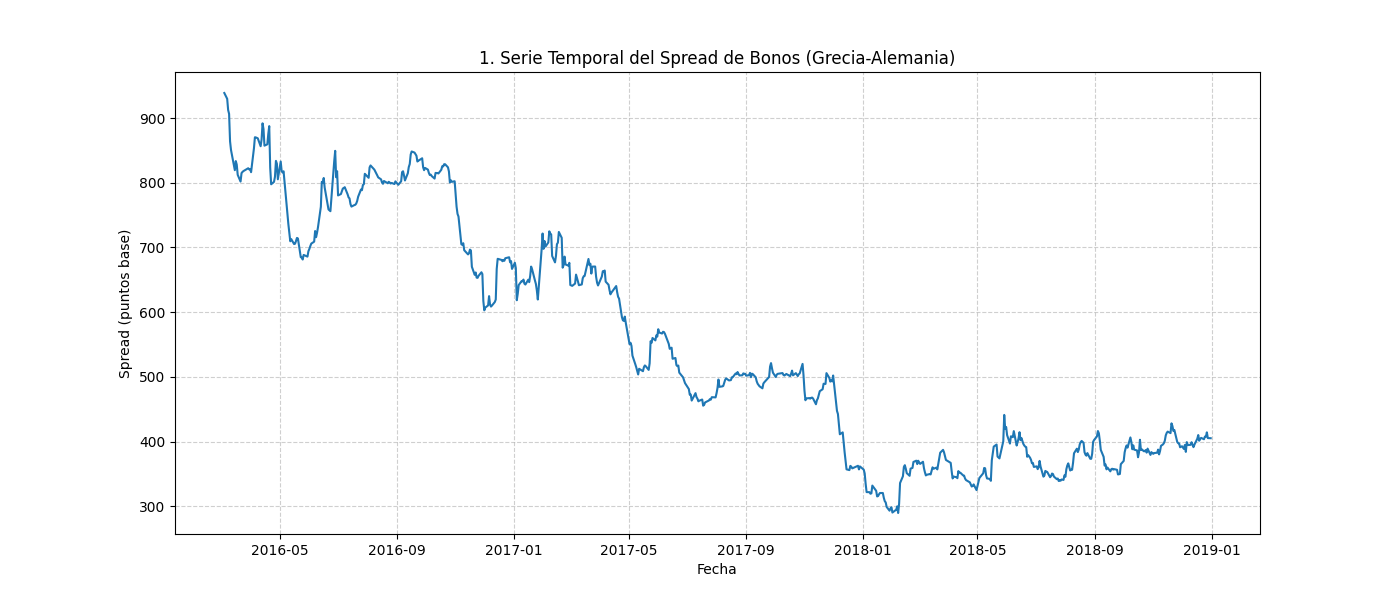
\includegraphics[width=0.8\linewidth]{../image/1_Serie_Temporal_Spread.png}
    \caption{Serie temporal del spread Grecia-Alemania}
    \label{fig:serie_spread}
\end{figure}

\begin{figure}[H]
    \centering
    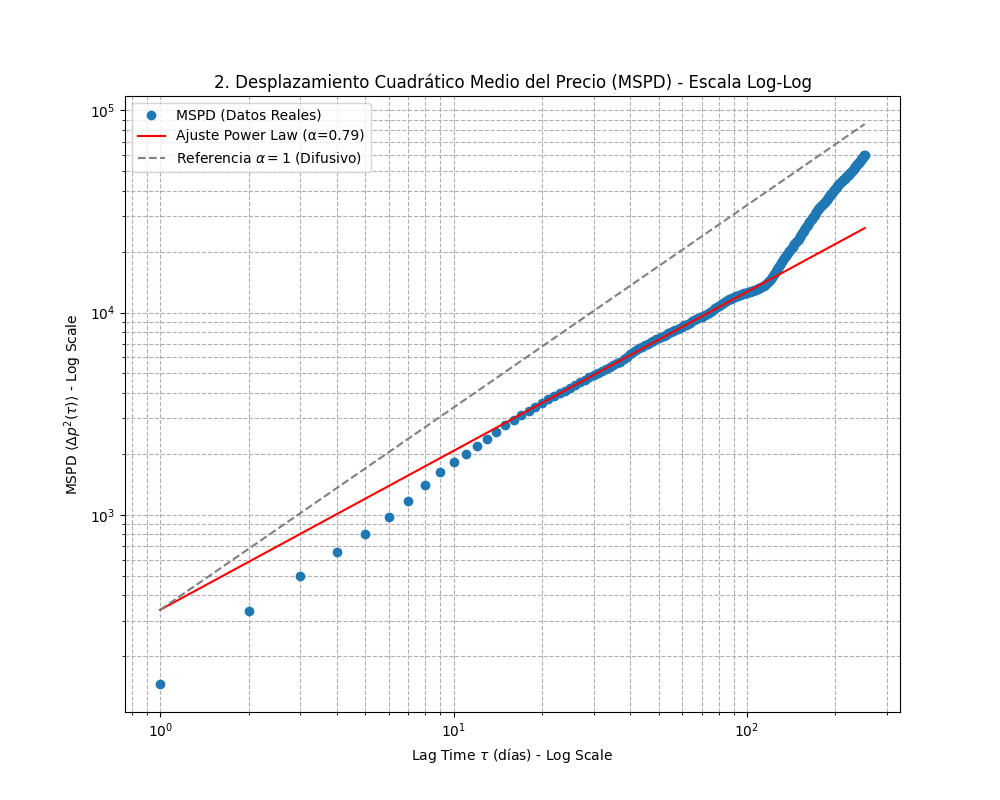
\includegraphics[width=0.8\linewidth]{../image/2_MSPD_Log_Log.png}
    \caption{MSPD en escala log-log}
    \label{fig:mspd_loglog}
\end{figure}

\subsection{Análisis}

El análisis de las gráficas generadas y los resultados del modelo de econofísica aplicado al spread Grecia-Alemania permite extraer varias conclusiones relevantes sobre la dinámica del sistema financiero durante el periodo analizado.

\subsubsection*{1. Serie Temporal del Spread (Figura~\ref{fig:serie_spread})}

La primera gráfica muestra la evolución temporal del spread entre los bonos de Grecia y Alemania. Se observa una marcada tendencia descendente desde niveles elevados (por encima de 900 puntos base) hacia valores más bajos, estabilizándose en torno a los 300--400 puntos base al final del periodo. Esta caída refleja la reducción progresiva del riesgo soberano percibido en Grecia tras los episodios más agudos de la crisis de deuda europea. Además, se aprecian fases de relativa estabilidad intercaladas con caídas abruptas, lo que sugiere la presencia de shocks y periodos de relajación lenta, características típicas de sistemas fuera de equilibrio.

\subsubsection*{2. MSPD en Escala Log-Log (Figura~\ref{fig:mspd_loglog})}

La segunda gráfica representa el desplazamiento cuadrático medio del precio (MSPD) en función del lag temporal $\tau$, en escala log-log. El ajuste de ley de potencia arroja un exponente $\alpha \approx 0.79$, claramente inferior al valor difusivo de referencia ($\alpha=1$). Esto indica que la dinámica del spread es \textbf{subdifusiva}: el sistema presenta memoria y relajación lenta, lo que es consistente con el comportamiento de arresto dinámico observado en sistemas vítreos o sobreenfriados en física estadística.

La desviación respecto a la línea difusiva confirma que el spread no sigue un paseo aleatorio clásico, sino que está sujeto a mecanismos de retención y persistencia, probablemente asociados a la incertidumbre y los efectos de la crisis financiera.

\subsubsection*{3. Modelo GARCH y Persistencia de la Volatilidad}

El intento de ajuste de un modelo GARCH(1,1) no ha convergido debido a la limitada cantidad de datos disponibles en el periodo analizado. Sin embargo, en contextos de arresto dinámico y baja volatilidad, es esperable que la persistencia de la volatilidad sea elevada, aunque difícil de estimar con series cortas. Para confirmar este efecto de memoria en la volatilidad, sería necesario ampliar el rango temporal y disponer de una serie más extensa.

\subsubsection*{4. Conclusión Integrada}

El modelo de econofísica aplicado ha permitido cuantificar la dinámica del spread Grecia-Alemania, mostrando evidencia clara de \textbf{subdifusión} y memoria en el sistema financiero durante la crisis. El exponente $\alpha < 1$ es consistente con la presencia de fases de relajación lenta y arresto dinámico, tal como predice la teoría de econofísica para mercados en tensión. Para obtener resultados más robustos y generalizables, es imprescindible analizar la serie completa que cubra todo el periodo de crisis (2009--2021), lo que permitiría confirmar la persistencia de la dinámica subdifusiva y caracterizar mejor los mecanismos de memoria en el mercado de deuda soberana europea.



% \printbibliography[heading=bibintoc]

% -------------------- Apéndices --------------------
% \begin{appendices}
% \section{Material suplementario}
% Información adicional, cuestionarios, resultados complementarios.
% \end{appendices}

% -------------------- Ejemplo de archivo .bib --------------------
% Crea un archivo llamado 'bibliografia.bib' en el mismo directorio con entradas como:
%
% @article{ejemplo2020,
%   author = {Apellido, Nombre and Otro, Nombre},
%   title = {Título del artículo},
%   journal = {Revista Ejemplo},
%   year = {2020},
%   volume = {10},
%   number = {2},
%   pages = {123--130},
% }
%
% -------------------- FIN --------------------
\end{document}
